\documentclass[11pt, a4paper, oneside]{scrreprt}

\usepackage[utf8]{inputenc}
\usepackage[T1]{fontenc}
\usepackage{lmodern}
\usepackage{microtype}
\usepackage{geometry}
\geometry{margin=2.5cm}

\usepackage{setspace}
\onehalfspacing

\usepackage[dvipsnames]{xcolor}
\definecolor{accent}{HTML}{004F9F}

\addtokomafont{chapter}{\color{accent}}
\addtokomafont{section}{\color{accent}}
\addtokomafont{subsection}{\color{accent}}

\usepackage{graphicx}
\usepackage{amsmath,amsfonts,amssymb}
\usepackage{booktabs}
\usepackage{siunitx}
\sisetup{detect-all}
\usepackage{caption}
\usepackage{subcaption}
\usepackage{enumitem}
\usepackage{xstring}
\usepackage{catchfile}

% -------------------------------------------------------
%  hyperref customization
% -------------------------------------------------------
\usepackage[
  pdfauthor={STEM Development Team},
  pdftitle={STEM Benchmark Report},
  colorlinks=true,
  linkcolor=accent,
  urlcolor=accent,
  citecolor=accent
]{hyperref}

% -------------------------------------------------------
%  header and footer
% -------------------------------------------------------
\usepackage{fancyhdr}
\renewcommand{\chaptermark}[1]{\markboth{\thechapter}{}}
\pagestyle{fancy}
\fancyhf{}
\lhead{\small{STEM Benchmark Report}}
\rhead{\small{Chapter~\thechapter}}
\cfoot{\small{\thepage}}

% -------------------------------------------------------
%  STEM version from python package
% -------------------------------------------------------
\newcommand{\versionfile}{../stem/__version__.py}
\CatchFileDef{\versionpyraw}{\versionfile}{}
\StrBehind{\versionpyraw}{__version__ = "}[\versiontmp]
\StrBefore{\versiontmp}{"}[\versionparsed]
\newcommand{\STEMversion}{\versionparsed}


% -------------------------------------------------------
%  for git hash
% -------------------------------------------------------
% Based on this: https://gist.github.com/kbjarkefur/88820e5a5365b3f707b6b20aee57cf8a
\newcommand{\gitfolder}{../.git}             % Relative path to .git folder from .tex file
\CatchFileDef{\headfull}{\gitfolder/HEAD}{}              % Get path to head file for checked out branch
\StrGobbleRight{\headfull}{1}[\head]                      % Remove end of line character
\StrBehind[2]{\head}{/}[\branch]                          % Parse out the path only
\CatchFileDef{\commit}{\gitfolder/refs/heads/\branch}{}  % Get the content of the branch head
\StrGobbleRight{\commit}{1}[\commithash]                  % Remove end of line character

% Define the hash
\newcommand{\commiturl}{\commithash}
\newcommand{\commitfont}[1]{\textsf{#1}}


% -------------------------------------------------------
%  paragraph style
% -------------------------------------------------------
\setlength{\parindent}{0pt}
\setlength{\parskip}{0.8em}

% -------------------------------------------------------
%  title page
% -------------------------------------------------------
\newcommand{\reporttitle}{
    \begin{titlepage}
    \centering
    \vspace*{2cm}
    {\Huge\bfseries STEM Benchmark Test Report \\[1.5em]}
    \rule{\textwidth}{0.5pt} \\[1.5em]
    {\Large Numerical Accuracy and Validation Results}\\[4em]
    {\Large \textbf{STEM Development Team}}\\[1em]
    \today
    \vfill
    \commitfont{Version} \commitfont{\STEMversion: \commiturl}
    \end{titlepage}
}

% % -------------------------------------------------------
% %  draft watermark
% % -------------------------------------------------------
% \usepackage{draftwatermark}
% \SetWatermarkText{DRAFT}
% \SetWatermarkScale{1}
% \SetWatermarkColor[HTML]{B0B0B0}


% -------------------------------------------------------
%  document
% -------------------------------------------------------
\begin{document}

\reporttitle
\tableofcontents
\clearpage

\chapter*{Summary}
\addcontentsline{toc}{chapter}{Summary} % include in ToC
This report presents the validation and benchmarking of the STEM model through a comprehensive set of numerical
test cases.
The objective of this benchmark study is to verify the numerical accuracy, robustness, and consistency of the
software by comparing its results against analytical solutions and well-established reference
problems from the literature.

The benchmark suite covers a broad range of dynamic and static problems relevant to geotechnical
and structural dynamics. These include single degree-of-freedom oscillators, one-dimensional wave propagation
with and without absorbing boundaries, dynamic and static loading of beams, wave propagation in elastic half-spaces,
strip and point load problems, and the dynamic response of a dam structure.
Both two-dimensional and three-dimensional model formulations are considered where appropriate
to assess consistency and convergence.

The results confirm that STEM provides reliable and accurate numerical solutions for a wide range of soil-structure
interaction and vibration problems. Together with its extensive automated test suite, these benchmarks
demonstrate the suitability of STEM as an open, transparent, and robust modelling tool for the analysis of
railway-induced vibrations and related geotechnical dynamic applications.
\clearpage

% ==============================================================================================
\chapter{Introduction}
% ==============================================================================================

This document provides a validation overview for the STEM (Soil and Track System Modeling Tool) software,
a Python-based numerical model designed to simulate railway-induced vibrations using the Finite Element Method (FEM).
The objective is to validate numerical accuracy through comparison against analytical solutions and
established benchmark results.

STEM is an open-source Python toolkit to model, simulate, and analyse railway-induced vibrations in
soil-track systems. It builds finite element models, generates meshes, writes Kratos Multiphysics input files,
runs multi-stage geotechnical and structural analyses, and collects results for verification and visualization.

STEM is an open and transparent model that allows users to model railway induced vibrations and test the
effect of mitigation techniques.

Besides the tests presented in this report, STEM is continuously tested through an extensive suite of automated tests.
All the tests are run on Windows and Linux systems on multiple cores, ensuring consistent cross-platform behaviour,
reliable concurrency performance, and early detection of environment-specific issues.
The tests include:

\begin{itemize}[noitemsep,topsep=0pt,parsep=0pt,partopsep=0pt]
    \item \textbf{Unit Tests}: Verify the correctness of individual functions and classes (e.g., mesh generation,
        load application).
    \item \textbf{Benchmarks}: Validate the integrated system against known physical phenomena, analytical solutions,
        or established engineering scenarios.
    % \item \textbf{Validation}: Verify the results of STEM against experimental results.
    \item \textbf{Extensive test suite} available in Kratos Multiphysics, in which 2401 unit tests and 1435 benchmark
        tests are run.
\end{itemize}

In the following chapters, we present a series of benchmark tests that assess the numerical accuracy of STEM.
Each chapter corresponds to a benchmark configuration, including the mathematical model, the numerical approach,
and the result comparison.

% ==============================================================================================
\chapter{Single degree of freedom} \label{ch:sdof}
% ==============================================================================================

% ----------------------------------------------------------------------------------------------
\section{Introduction}
% ----------------------------------------------------------------------------------------------

This benchmark compares the STEM numerical solution against the analytical solution, for a single degree of freedom
mass--spring--damper oscillator.
The STEM numerical response is compared with the analytical solution of the linear oscillator subjected to the
sudden application of its self-weight.
The analytical solution is described in~\cite{Verruijt_2010}.

% ----------------------------------------------------------------------------------------------
\section{Model Description}
% ----------------------------------------------------------------------------------------------

% ..............................................................................................
\subsection{Geometry and loading}
% ..............................................................................................
The model consists of a mass--spring--damper sytem, where the damper is connected in parallel to the spring.
The system is subjected to a step load equal to the self-weight of the mass, applied at \qty{0}{\second}.
Figure~\ref{fig:sdof_model} illustrates the configuration of the single degree of freedom oscillator.

\begin{figure}
    \centering
    \includegraphics[width=0.75\textwidth]{sdof/sdof.pdf}
    \caption{Geometry of the single degree of freedom oscillator.}
    \label{fig:sdof_model}
\end{figure}

% ..............................................................................................
\subsection{Materials and numerical parameters}
% ..............................................................................................
The spring--damper element follows a linear elastic constitutive law. The mass is
introduced through a nodal concentrated element. The parameters employed in the calculation are:

\begin{itemize}[noitemsep,topsep=0pt,parsep=0pt,partopsep=0pt]
	\item Spring stiffness: \qty{10}{\kilo\newton\per\meter},
	\item Damping coefficient: \qty{100}{\newton\second\per\meter},
	\item Concentrated mass: \qty{10}{\kilogram},
	\item Gravity acceleration: \qty{9.81}{\meter\per\second\squared}.
\end{itemize}

The dynamic analysis has the duration of \qty{1.0}{\second} with a time step of \qty{0.001}{\second}.
The equations of motion are integrated with the Newmark scheme~\cite{Newmark_1959} using the average
acceleration parameters $\beta = 0.25$ and $\gamma = 0.5$. A

% ----------------------------------------------------------------------------------------------
\section{Results}
% ----------------------------------------------------------------------------------------------
Figure~\ref{fig:sdof_results} shows the vertical displacement history of the mass obtained with STEM and compares
it against the analytical solution. The results show a perfect agreement between the numerical and analytical results.

\begin{figure}[h]
	\centering
	\includegraphics[width=0.8\textwidth]{sdof/time_history.pdf}
	\caption{Comparison between the STEM and analytical vertical for the displacement of the single degree of freedom.}
	\label{fig:sdof_results}
\end{figure}


% ==============================================================================================
\chapter{One-dimensional wave propagation in an elastic column} \label{ch:one_dim_wave_prop}
% ==============================================================================================

% ----------------------------------------------------------------------------------------------
\section{Introduction}
% ----------------------------------------------------------------------------------------------
This benchmark compares the STEM numerical solution against the analytical solution,
for the one dimensional wave propagation in a vertical elastic soil column, subjected to a surface load.

The analytical solution is presented in~\cite{Verruijt_2010}.
The analytical solution provides closed-form expressions for the vertical velocity along the column,
enabling a direct time-history comparison against the numerical model.

% ----------------------------------------------------------------------------------------------
\section{Model Description}
% ----------------------------------------------------------------------------------------------

% ..............................................................................................
\subsection{Geometry, mesh and loading}
% ..............................................................................................
Two soil domains are modelled, a two-dimensional and a three-dimensional continuum representing vertical columns.
The two-dimensional column is modelled with a height of \qty{10}{\meter} and a width of \qty{0.25}{\meter}.
The three-dimensional column is modelled with a height of \qty{10}{\meter} and a square cross-section of
\qty{0.25}{\meter} by \qty{0.25}{\meter}.
The columns are aligned with the $y$-axis, so that wave propagation is essentially one-dimensional along
the vertical direction.

For the two-dimensional column, the soil is discretised with second-order triangular elements, for the three-dimensional
column, the soil is discretised with second-order tetrahedral elements.
In both cases, an average element size of \qty{0.10}{\meter} is adopted.
An overview of the geometries and meshes adopted for the analysis is shown in
Figure~\ref{fig:one_dim_wave_mesh}.
A vertical distributed load is applied on the entire top face of the column. The load acts in compression along
the $y$-direction and is applied as a step function in time:

\begin{equation}
	p(t) =
	\begin{cases}
		0, & t < \qty{0}{\second}, \\
		\qty{-1000}{\kilo\newton\per\meter\squared}, & t \geq \qty{0}{\second}.
	\end{cases}
\end{equation}

The four vertical faces are restrained only in the horizontal directions, thereby allowing vertical motion
similar to a one-dimensional situation.
In the two-dimensional case, the side lines are restrained in the horizontal direction.
In the three-dimensional case, the four vertical faces are restrained only in the horizontal directions,
thereby allowing vertical motion similar to a one-dimensional situation.

\begin{figure}
	\centering
	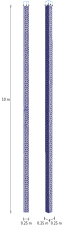
\includegraphics[width=0.20\textwidth]{one_d_abs_boundary/one_d_column_mesh.pdf}
	\caption{Geometry and mesh adopted for the one-dimensional wave propagation benchmark. }
	\label{fig:one_dim_wave_mesh}
\end{figure}

% ..............................................................................................
\subsection{Materials and numerical parameters}
% ..............................................................................................
The soil is modelled as a one-phase continuum with a linear elastic constitutive law, with the
following parameters:

\begin{itemize}[noitemsep,topsep=0pt,parsep=0pt,partopsep=0pt]
	\item Young's modulus: \qty{50}{\mega\pascal},
	\item Poisson ratio: \qty{0.3}{},
	\item Solid density: \qty{2000}{\kilogram\per\meter\cubed}.
\end{itemize}

Material damping is included via Rayleigh damping, with parameters that provide a damping ratio of
\qty{0.5}{\percent} at \qty{1}{\hertz} and \qty{80}{\hertz}.

The dynamic analysis is performed over a \qty{0.20}{\second} time window, with a time step of \qty{0.001}{\second}.
The system of equations is solved using the Newmark time integration~\cite{Newmark_1959} scheme with
parameters $\beta = 0.25$ and $\gamma = 0.5$.


% ----------------------------------------------------------------------------------------------
\section{Results}
% ----------------------------------------------------------------------------------------------
Figure~\ref{fig:one_dim_wave_results} presents the time histories of the
vertical velocity at three points located at: \qty{2.5}{\meter}, \qty{5}{\meter} and \qty{7.5}{\meter}
along the height of the column.
The figure compares the numerical STEM results against the analytical solution of the one-dimensional wave equation.

The arrival times of the incident and reflected waves at the observation point match closely between the numerical
and analytical solutions.
The amplitudes of the displacement and velocity pulses also show very good agreement, with small differences
attributable to the introduced material and numerical damping.

\begin{figure}[h]
	\centering
	\includegraphics[width=0.8\textwidth]{one_dim_wave_prop/time_history.pdf}
	\caption{Comparison of the vertical velocity time histories at three points located at:
    (a) \qty{2.5}{\meter}, (b) \qty{5}{\meter} and (c) \qty{7.5}{\meter}
	along the column height.}
	\label{fig:one_dim_wave_results}
\end{figure}


% ==============================================================================================
\chapter{One-dimensional wave propagation in an elastic column with an absorbing boundary} \label{ch:one_dim_abs_boundary}
% ==============================================================================================

% ----------------------------------------------------------------------------------------------
\section{Introduction}
% ----------------------------------------------------------------------------------------------
This benchmark compares the STEM numerical solution against the analytical solution,
for the one dimensional wave propagation in a vertical elastic soil column with an absorbing boundary at the bottom,
subjected to a surface load.

The analytical solution for 1D wave propagation on infinite columns is presented in~\cite{Verruijt_2010}.
The analytical solution provides closed-form expressions for the vertical velocity along the column,
enabling a direct time-history comparison against the numerical model.

% ----------------------------------------------------------------------------------------------
\section{Model Description}
% ----------------------------------------------------------------------------------------------

% ..............................................................................................
\subsection{Geometry, mesh and loading}
% ..............................................................................................
Two soil domains are modelled, a two-dimensional and a three-dimensional continuum representing vertical columns.
The two-dimensional column is modelled with a height of \qty{10}{\meter} and a width of \qty{0.25}{\meter}.
The three-dimensional column is modelled with a height of \qty{10}{\meter} and a square cross-section of
\qty{0.25}{\meter} by \qty{0.25}{\meter}.
The columns are aligned with the $y$-axis, so that wave propagation is essentially one-dimensional along
the vertical direction.

For the two-dimensional column, the soil is discretised with second-order triangular elements, for the three-dimensional
column, the soil is discretised with second-order tetrahedral elements.
In both cases, an average element size of \qty{0.10}{\meter} is adopted.
An overview of the geometries and meshes adopted for the analysis is shown in
Figure~\ref{fig:one_dim_wave_abs_mesh}.
A vertical distributed load is applied on the entire top face of the column. The load acts in compression along
the $y$-direction and is applied as a step function in time:

\begin{equation}
	p(t) =
	\begin{cases}
		0, & t < \qty{0}{\second}, \\
		\qty{-1000}{\kilo\newton\per\meter\squared}, & t \geq \qty{0}{\second}.
	\end{cases}
\end{equation}

The base of the column has an absorbing boundary condition, absorbing all waves in the normal direction.
In the two-dimensional case, the side lines are restrained in the horizontal direction.
In the three-dimensional case, the four vertical faces are restrained only in the horizontal directions,
thereby allowing vertical motion similar to a one-dimensional situation.

\begin{figure}
	\centering
	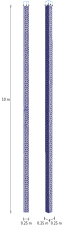
\includegraphics[width=0.2\textwidth]{one_d_abs_boundary/one_d_column_mesh.pdf}
	\caption{Geometry and mesh adopted for the one-dimensional
	wave propagation with absorbing boundary benchmark. }
	\label{fig:one_dim_wave_abs_mesh}
\end{figure}

% ..............................................................................................
\subsection{Materials and numerical parameters}
% ..............................................................................................
The soil is modelled as a one-phase continuum with a linear elastic constitutive law, with the
following parameters:

\begin{itemize}[noitemsep,topsep=0pt,parsep=0pt,partopsep=0pt]
	\item Young's modulus: \qty{50}{\mega\pascal},
	\item Poisson ratio: \qty{0.3}{},
	\item Solid density: \qty{2700}{\kilogram\per\meter\cubed},
	\item Porosity: 0.3.
\end{itemize}


Material damping is included via Rayleigh damping, with parameters that provide a damping ratio of
\qty{0.5}{\percent} at \qty{1}{\hertz} and \qty{80}{\hertz}.

The dynamic analysis is performed over a \qty{0.20}{\second} time window, with a time step of \qty{0.001}{\second}.
The system of equations is solved using the Newmark time integration~\cite{Newmark_1959} scheme with
parameters $\beta = 0.25$ and $\gamma = 0.5$.


% ----------------------------------------------------------------------------------------------
\section{Results}
% ----------------------------------------------------------------------------------------------
Figure~\ref{fig:one_dim_wave_abs_boundary_results} presents the time histories of the
vertical velocity at a point located at:  \qty{2.5}{\meter}, \qty{5}{\meter} and \qty{7.5}{\meter}
along the height of the column.
The figure compares the numerical STEM results against the analytical solution of the one-dimensional wave equation with
absorbing boundary.

The arrival time of the incident wave at the observation point matches closely between the numerical
and analytical solution. It can also be observed that there is no reflection from the bottom boundary,
indicating that the absorbing boundary condition is functioning as intended.
The amplitude of the velocity pulse also shows very good agreement.

\begin{figure}[h]
	\centering
	\includegraphics[width=0.8\textwidth]{one_d_abs_boundary/time_history.pdf}
	\caption{Comparison of the vertical velocity time history at \qty{5}{\meter} along the column height.}
	\label{fig:one_dim_wave_abs_boundary_results}
\end{figure}

% ==============================================================================================
\chapter{Distributed load on simply supported beam} \label{ch:simply_supported_beam}
% ==============================================================================================

% ----------------------------------------------------------------------------------------------
\section{Introduction}
% ----------------------------------------------------------------------------------------------

This benchmark compares the STEM numerical solution against the analytical solution for the dynamic response of a
simply supported beam subjected to a uniformly distributed load that is suddenly removed.

The STEM numerical response is compared with the analytical solution in terms of the first-mode period of vibration
and the maximum and minimum mid-span displacements.

The first-mode period of vibration, $T_{1}$ is calculated as:

\begin{equation}
    T_{1} = \frac{1}{f_{1}},
\end{equation}

\begin{equation}
    f_{1} = \frac{1}{2 \pi} \left( \frac{\pi}{L} \right)^2 \sqrt{\frac{E I}{\rho A}},
\end{equation}

Where $f_{1}$ is the first-mode natural frequency, $L$ is the length of the beam, $E$ is the Young's modulus, $I$ is
the moment of inertia, $\rho$ is the density and $A$ is the cross-sectional area.

The maximum and minimum mid-span displacements, $u_{max}$ and $u_{min}$, respectively, are calculated as:
\begin{equation}
    u_{max} = \frac{q L^{4}}{384 E I}
\end{equation}
\begin{equation}
    u_{min} = -u_{max}
\end{equation}

Where $q$ is the magnitude of the distributed load.


% ----------------------------------------------------------------------------------------------
\section{Model Description}
% ----------------------------------------------------------------------------------------------

% ..............................................................................................
\subsection{Geometry and loading}
% ..............................................................................................
The model consists of a simply supported beam with a length of \qty{25}{\meter}. The beam is initially subjected to a
uniformly distributed load of \qty{1}{\newton\per\meter}. The dynamic response is analysed following the sudden
removal of the distributed load. The analysis is performed for both 2D and 3D configurations.

Figure~\ref{fig:simply_supported_beam_model} illustrates the geometry, boundary conditions and loading of the
simply supported beam.

\begin{figure}
    \centering
    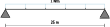
\includegraphics[width=0.8\textwidth]{simply_supported_beam/simply_supported_beam.pdf}
    \caption{Geometry, boundary conditions and loading of the simply supported beam.}
    \label{fig:simply_supported_beam_model}
\end{figure}

% ..............................................................................................
\subsection{Materials and numerical parameters}
% ..............................................................................................
The simply supported beam is modelled using Euler-Bernoulli beam elements. The beam properties used in analysis are:

\begin{itemize}[noitemsep,topsep=0pt,parsep=0pt,partopsep=0pt]
	\item Young's modulus: \qty{316628.699}{\newton\per\meter\squared},
	\item Poisson ratio: \qty{0.3}{},
	\item Density: \qty{1}{\kilogram\per\meter\cubed},
	\item Cross-sectional area: \qty{0.5}{\meter\squared},
    \item Moment of inertia: \qty{1}{\meter\tothe{4}},
\end{itemize}

The beam is discretised using beam elements with an element size of \qty{0.3125}{\meter}.

The dynamic analysis has a duration of \qty{2}{\second} with a time step of \qty{0.00125}{\second}.
The equations of motion are integrated with the Newmark scheme~\cite{Newmark_1959} using the average
acceleration parameters $\beta = 0.25$ and $\gamma = 0.5$. No damping is considered in the analysis.

% ----------------------------------------------------------------------------------------------
\section{Results}
% ----------------------------------------------------------------------------------------------
Figure~\ref{fig:simply_supported_beam_results} shows the vertical displacement history at the mid-span of the beam
obtained using STEM in both two and three-dimensional, and compares it with the analytical solution. The results show that the
first-mode period of vibration and the maximum and minimum mid-span displacements obtained with STEM are in agreement
with the analytical solution.

\begin{figure}[h]
	\centering
	\includegraphics[width=0.8\textwidth]{simply_supported_beam/simply_supported_beam_results.pdf}
	\caption{Comparison between the STEM and analytical vertical displacement at mid-span of the simply supported beam.}
	\label{fig:simply_supported_beam_results}
\end{figure}


% ==============================================================================================
\chapter{Moving load on a beam} \label{ch:moving_load_beam}
% ==============================================================================================

% ----------------------------------------------------------------------------------------------
\section{Introduction}
% ----------------------------------------------------------------------------------------------

This benchmark compares the STEM numerical solution against the analytical solution for the dynamic response of a
simply supported beam subjected to a moving load, traveling at a constant speed from one end of the beam to the other.

The STEM numerical response is compared with the analytical solution, presented in ~\cite[Chapter 1.3.2.2]{Fryba_1972}.
The analytical solution provides closed-form expressions for the vertical displacement along the beam, enabling a
direct time-history comparison against the numerical model.


% ----------------------------------------------------------------------------------------------
\section{Model Description}
% ----------------------------------------------------------------------------------------------

% ..............................................................................................
\subsection{Geometry and loading}
% ..............................................................................................
The model consists of a simply supported beam with a length of \qty{25}{\meter}. The beam is subjected to
a moving vertical point load with a magnitude of \qty{1}{\kilo\newton}. The load travels at a constant speed of
\qty{10}{\meter\per\second}, starting at the left support.
The analysis is performed for both 2D and 3D configurations.

Figure~\ref{fig:moving_load_on_beam_model} illustrates the geometry, boundary conditions and loading of the
simply supported beam with the moving load.

\begin{figure}
    \centering
    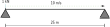
\includegraphics[width=0.8\textwidth]{moving_load_on_beam/simply_supported_beam_with_moving_load.pdf}
    \caption{Geometry, boundary conditions and loading of the simply supported beam.}
    \label{fig:moving_load_on_beam_model}
\end{figure}

% ..............................................................................................
\subsection{Materials and numerical parameters}
% ..............................................................................................
The simply supported beam is modelled using Euler-Bernoulli beam elements. The beam properties used in analysis are:

\begin{itemize}[noitemsep,topsep=0pt,parsep=0pt,partopsep=0pt]
	\item Young's modulus: \qty{210e9}{\newton\per\meter\squared},
	\item Poisson ratio: \qty{0.3}{},
	\item Density: \qty{7850}{\kilogram\per\meter\cubed},
	\item Cross-sectional area: \qty{0.01}{\meter\squared},
    \item Moment of inertia: \qty{0.0001}{\meter\tothe{4}},
\end{itemize}

The beam is discretised using beam elements with an element size of \qty{2.5}{\meter}.

The dynamic analysis has a duration of \qty{2.5}{\second} with a time step of \qty{0.0025}{\second}.
The equations of motion are integrated with the Newmark scheme~\cite{Newmark_1959} using the average
acceleration parameters $\beta = 0.25$ and $\gamma = 0.5$. No damping is considered in the analysis.

% ----------------------------------------------------------------------------------------------
\section{Results}
% ----------------------------------------------------------------------------------------------
Figure~\ref{fig:moving_load_on_beam_results} shows the vertical displacement history at the mid-span of the beam
obtained using STEM in both 2D and 3D, and compares it with the analytical solution. The results show that the
mid-span deflections obtained with STEM are in agreement
with the analytical solution.

\begin{figure}[h]
	\centering
	\includegraphics[width=0.8\textwidth]{moving_load_on_beam/moving_load_on_beam_results.pdf}
	\caption{Comparison between the STEM and analytical vertical displacement at mid-span of the simply supported beam.}
	\label{fig:moving_load_on_beam_results}
\end{figure}


% ==============================================================================================
\chapter{Moving load on an elastic halfspace} \label{ch:moving_load_halfspace}
% ==============================================================================================

% ----------------------------------------------------------------------------------------------
\section{Introduction}
% ----------------------------------------------------------------------------------------------
This benchmark compares the STEM numerical solution against the analytical solution,
for a moving load travelling on an elastic halfspace.

The analytical solution is presented in~\cite{Liao_Teng_Yeh_2005}.
The analytical solution provides closed-form expressions for the vertical displacement below the surface of the
halfspace, enabling a direct time-history comparison against the numerical model.

% ----------------------------------------------------------------------------------------------
\section{Model Description}
% ----------------------------------------------------------------------------------------------

% ..............................................................................................
\subsection{Geometry, mesh and loading}
% ..............................................................................................
The soil domain is modelled as a three-dimensional block representing the halfspace, with the following dimensions:
height \qty{10}{\meter}, width \qty{10}{\meter} and length \qty{20}{\meter}.
The soil is discretised with second-order tetrahedral elements, using an average element size of \qty{0.50}{\meter}.
An overview of the geometry and mesh adopted for the analysis is shown in
Figure~\ref{fig:moving_load_halfspace_mesh}.

The moving load is modelled as a vertical point load travelling along the z-direction at a constant speed of
\qty{10}{\meter\per\second}.
The load has a magnitude of \qty{1000}{\kilo\newton}.

The nodes at the sides of the soil have absorbing boundaries at the free ends, and with fixed boundary conditions
on the perpendicular plane along the axis of symmetry.
At the bottom the soil is assumed to be fixed.


\begin{figure}
	\centering
	\includegraphics[width=0.75\textwidth]{moving_load_halfspace/mesh.pdf}
	\caption{Geometry and mesh adopted for the moving load on an elastic halfspace benchmark.}
	\label{fig:moving_load_halfspace_mesh}
\end{figure}

% ..............................................................................................
\subsection{Materials and numerical parameters}
% ..............................................................................................
The soil is modelled as a one-phase continuum with a linear elastic constitutive law, with the
following parameters:

\begin{itemize}[noitemsep,topsep=0pt,parsep=0pt,partopsep=0pt]
	\item Young's modulus: \qty{30}{\mega\pascal},
	\item Poisson ratio: \qty{0.2}{},
	\item Solid density: \qty{2000}{\kilogram\per\meter\cubed},
\end{itemize}

% The material damping is set to zero, in order to allow a direct comparison against the analytical solution.
Material damping is included via Rayleigh damping, with parameters that provide a damping ratio of
\qty{1}{\percent} at \qty{1}{\hertz} and \qty{80}{\hertz}.

The dynamic analysis is performed over a \qty{1.5}{\second} time window, with a time step of \qty{0.01}{\second}.
The system of equations is solved using the Newmark time integration~\cite{Newmark_1959} scheme with
parameters $\beta = 0.25$ and $\gamma = 0.5$.


% ----------------------------------------------------------------------------------------------
\section{Results}
% ----------------------------------------------------------------------------------------------
Figure~\ref{fig:moving_load_halfspace_results} presents the time history of the
vertical displacement for a point located in the middle of the model at a depth of \qty{1}{\meter}
(coordinates (5, 5, -1)).
The figure compares the numerical STEM results against the analytical solution.
If follows that there is an agreement between both solutions, demonstrating the accuracy of the STEM
for this type of dynamic loading condition. The STEM solution exhibits some high frequency content,
which is not present in the analytical solution, and which are related to the domain truncation, and boundary conditions
adopted in the numerical model (the analytical solution assumes an infinite halfspace).

\begin{figure}[h]
	\centering
	\includegraphics[width=0.8\textwidth]{moving_load_halfspace/time_history.pdf}
	\caption{Comparison of the vertical displacement time history at a point located in the middle of the model at
	 a depth of \qty{1}{\meter} (coordinates (5, 5, -1)).}
	\label{fig:moving_load_halfspace_results}
\end{figure}


% ==============================================================================================
\chapter{Dynamic point load on elastic halfspace}\label{ch:pekeris}
% ==============================================================================================

% ----------------------------------------------------------------------------------------------
\section{Introduction}
% ----------------------------------------------------------------------------------------------
This benchmark compares the STEM numerical solution against the analytical solution
for a dynamic point load applied to the surface of an elastic half-space (known as the Lamb problem).

The analytical solution was derived by Pekeris and is detailed in~\cite{Verruijt_2010}.
The analytical solution provides closed-form expressions for the vertical displacement along the surface of the
half-space, enabling a direct time-history comparison against the numerical model.


% ----------------------------------------------------------------------------------------------
\section{Model Description}
% ----------------------------------------------------------------------------------------------

% ..............................................................................................
\subsection{Geometry, mesh and loading}
% ..............................................................................................
The point load was modelled in a three-dimensional domain representing an elastic half-space.
An overview of the geometry for the numerical analysis is shown in Figure~\ref{fig:3D_scheme}.
The soil has a width and length of \qty{10}{\meter} and depth of \qty{5}{\meter} and is subjected to a
compressive pulse load, $F(t)$, which is suddenly applied at the top edge:

\begin{equation}
    F(t) =
     \begin{cases}
    0, & \text{if } t<0\\
    \qty{-1000}{\kilo\newton}, & \text{if } t>0\\
    \end{cases}
\end{equation}


\begin{figure}
    \centering
    \includegraphics[width=0.75\textwidth]{lamb/mesh.pdf}
    \caption{Geometry, mesh and loading conditions for the three-dimensional wave propagation problem.}
    \label{fig:3D_scheme}
\end{figure}

The soil is discretised in second-order tetrahedral elements with size \qty{0.25}{\meter}.
Absorbing boundary conditions are applied at the free ends of the lateral boundaries, while fixed boundary
conditions are imposed on the perpendicular plane along the axis of symmetry.
At the bottom the soil is assumed to be fixed, simulating the existence of the top of bedrock that has a
significantly larger stiffness than the soil above.

% ..............................................................................................
\subsection{Materials and numerical parameters}
% ..............................................................................................
The soil is modelled as a one-phase continuum with a linear elastic constitutive law, with the
following parameters:

\begin{itemize}[noitemsep,topsep=0pt,parsep=0pt,partopsep=0pt]
    \item Young's modulus: \qty{30}{\mega\pascal},
    \item Poisson ratio: \qty{0.3},
    \item Density: \qty{2000}{\kilogram\per\meter\cubed}.
\end{itemize}

Material damping is included via Rayleigh damping, with parameters that provide a damping ratio of
\qty{0.01}{\percent} at \qty{1}{\hertz} and \qty{80}{\hertz}.

The dynamic analysis is performed over a \qty{0.08}{\second} time window, with a time step of \qty{0.001}{\second}.
The system of equations is solved using the Newmark time integration~\cite{Newmark_1959} scheme with
parameters $\beta = 0.25$ and $\gamma = 0.5$.

% ----------------------------------------------------------------------------------------------
\section{Results}
% ----------------------------------------------------------------------------------------------
Figure~\ref{fig:pekeris_results} presents the time histories of the vertical displacement for three
nodes, located at 1, 2 and~\qty{3}{\meter} from the load, located along the surface.
The figure compares the STEM results against the analytical solution.
If follows that there is an agreement between both solutions, demonstrating the accuracy of the STEM
for this type of dynamic loading condition. This is a notable difficult problem to solve numerically,
due to the steep gradients in stress and displacement that occur close to the point of application of the
load.

\begin{figure}[h]
    \centering
    \includegraphics[width=0.8\textwidth]{lamb/time_history.pdf}
    \caption{Comparison of the vertical displacement time histories at surface nodes located at:
     (a) \qty{1}{\meter}, (b) \qty{2}{\meter} and (c) \qty{3}{\meter} from the load.}
    \label{fig:pekeris_results}
\end{figure}

% ==============================================================================================
\chapter{Dynamic strip load elastic halfspace} \label{ch:strip_load_2D}
% ==============================================================================================

% ----------------------------------------------------------------------------------------------
\section{Introduction}
% ----------------------------------------------------------------------------------------------
This benchmark compares the STEM numerical solution against the analytical solution,
where a dynamic line load is applied along the surface of an elastic half-space discretised in a plane-strain setting.

The analytical solution is presented in~\cite{Verruijt_Brinkgreve_Li_2008}.
The analytical solution provides closed-form expressions for the vertical stress along the surface of the
half-space, enabling a direct time-history comparison against the numerical model.

% ----------------------------------------------------------------------------------------------
\section{Model Description}
% ----------------------------------------------------------------------------------------------

% ..............................................................................................
\subsection{Geometry, mesh and loading}
% ..............................................................................................
The analytical solution is formulated in plane-strain conditions. To mimic this, two analyses are performed:
a two-dimensional analysis representing a strip load in plane-strain conditions, and a three-dimensional
analysis representing a strip load in a full 3D setting, where the thickness in the out-of-plane direction is set to
\qty{1}{\meter} and the displacements are fixed in the out-of-plane direction. This allows to verify that the
three-dimensional solution converges to the analytical solution.

In the two-dimensional analysis, the soil domain is modelled as a
\qty{20}{\meter} (x-direction) by \qty{10}{\meter} (y-direction) soil layer,
modelled with second-order triangular elements.

In the three-dimensional analysis, the soil domain is modelled as  a \qty{20}{\meter} (x-direction) by \qty{10}{\meter}
(y-direction) soil layer, extruded to \qty{1}{\meter} thickness in the z-direction, and modelled with second-order
 tetrahedral elements.

Both analyses use a mesh with an average element size of \qty{0.15}{\meter}.

Figure~\ref{fig:strip_mesh} illustrates the geometry and mesh adopted for the analyses.

The strip load is applied at the surface with a width of \qty{1}{\meter}.
A downward line load with magnitude \qty{1e6}{\newton\per\meter} is applied instantaneously and kept
constant during the analysed time window:

\begin{equation}
    q(t) =
    \begin{cases}
        0, & t < 0, \\
        \qty{-1000}{\kilo\newton\per\meter}, & t \geq 0.
    \end{cases}
\end{equation}

The nodes at the bottom are fully fixed, while the two vertical sides are restrained only in the normal direction
(roller boundaries) to allow vertical and tangential movement.
In the three-dimensional case, the front and back surface are prevented from moving in the
out-of-plane direction, to simulate plane-strain conditions along the extrusion axis.

\begin{figure}
    \centering
    \begin{subfigure}[t]{0.49\textwidth}
        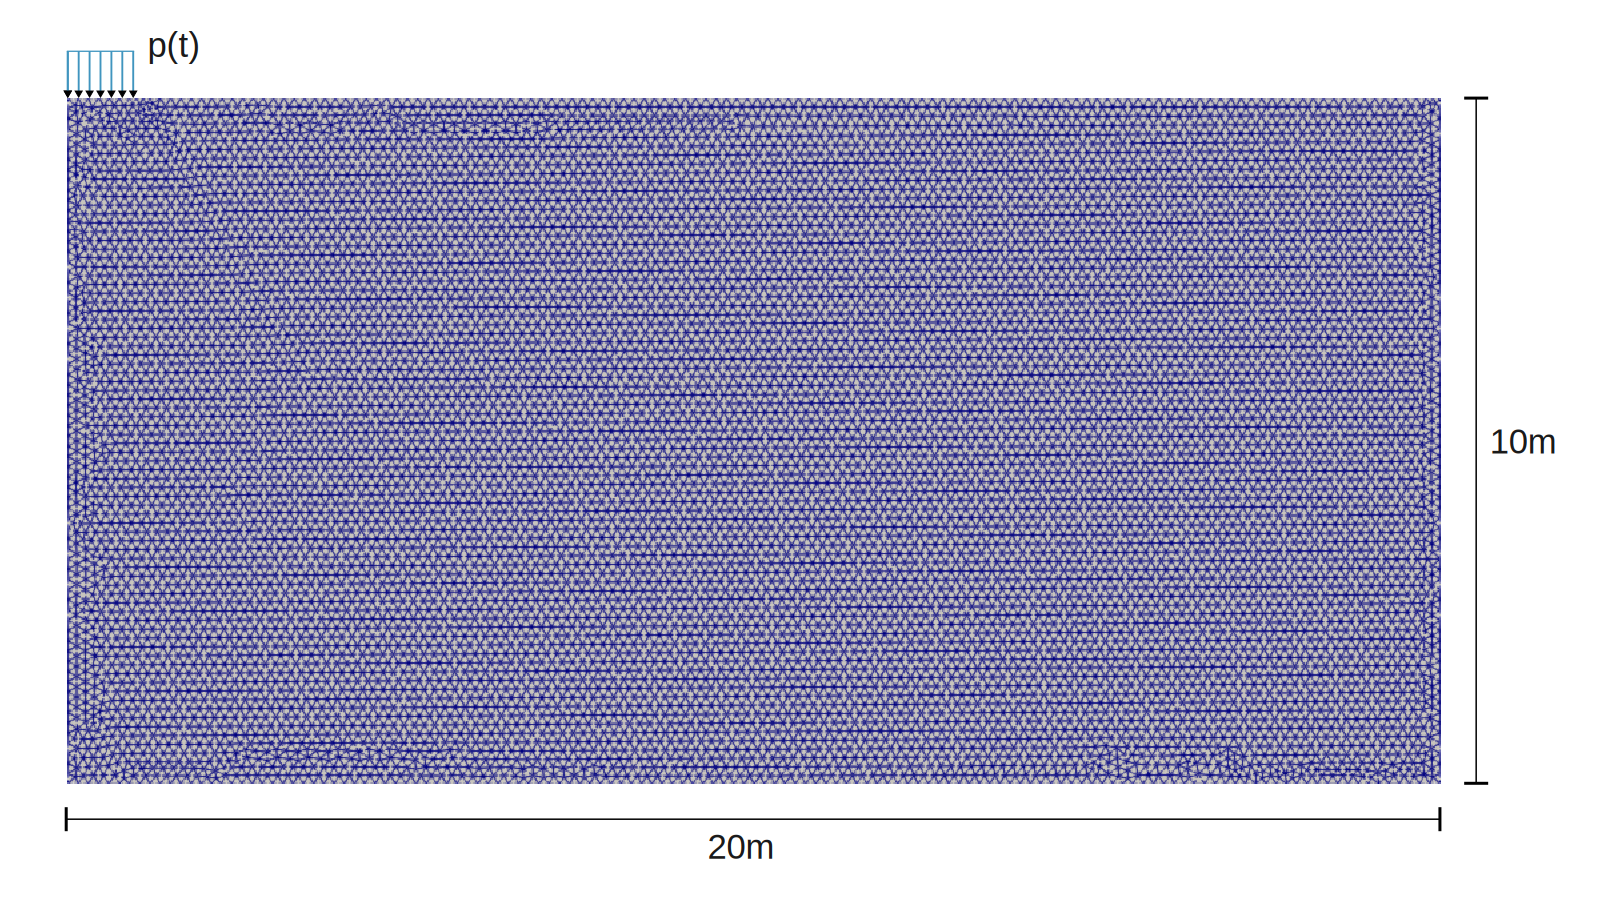
\includegraphics[width=\textwidth]{strip_load/mesh_2D.pdf}
    \caption{}
    \label{fig:strip_mesh_a}
    \end{subfigure}
    \begin{subfigure}[t]{0.49\textwidth}
        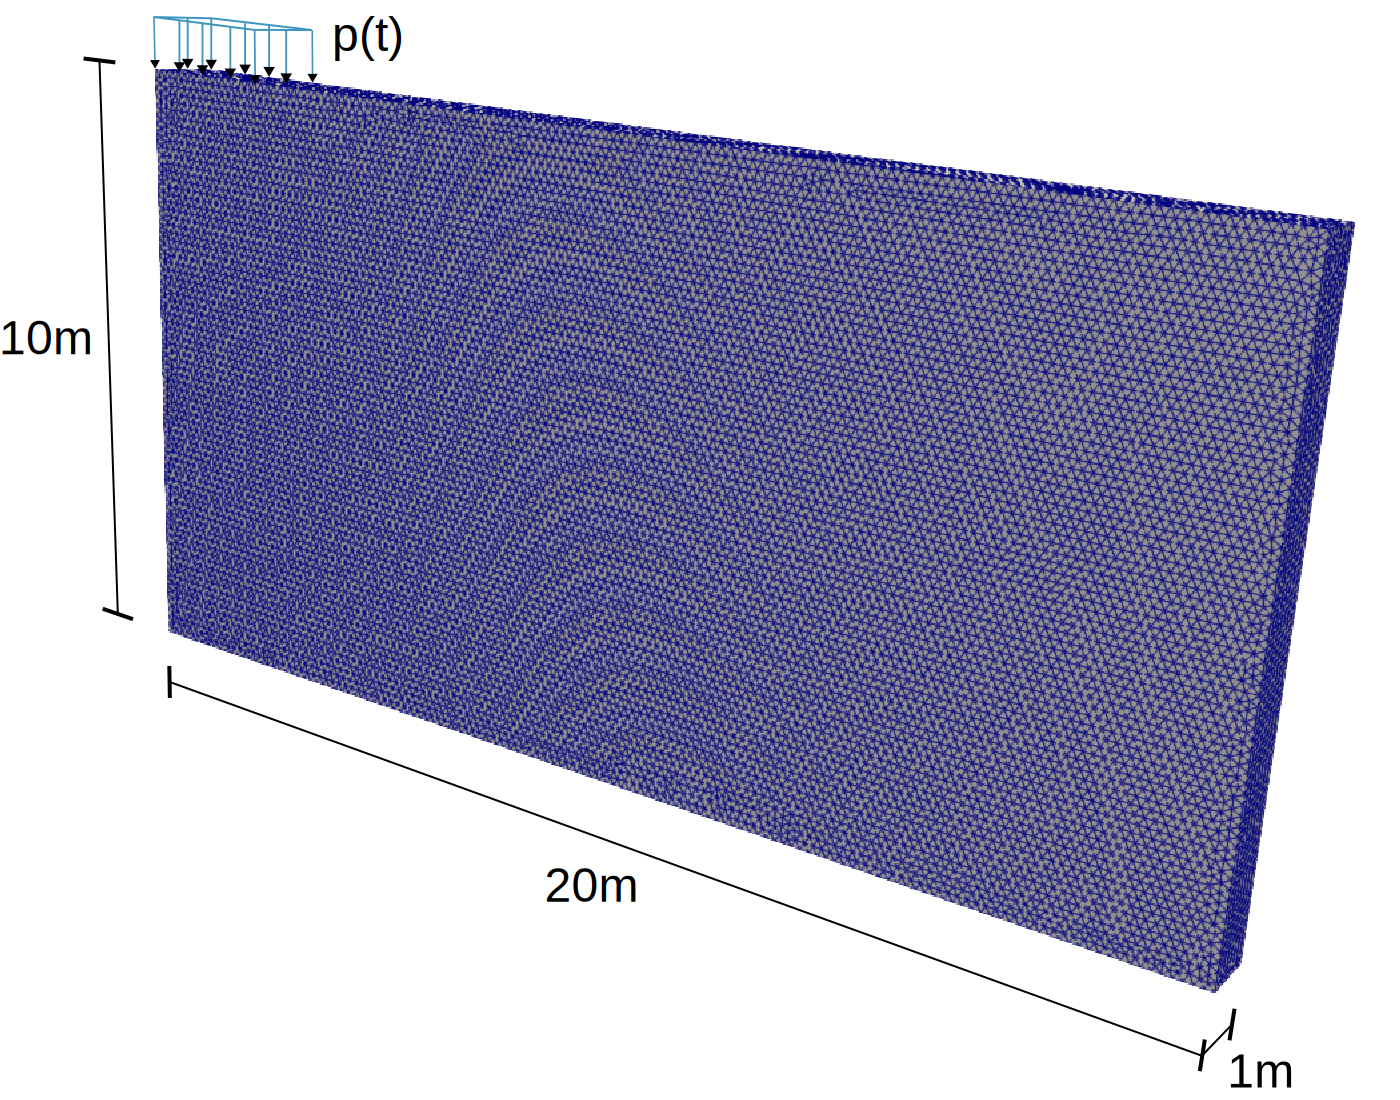
\includegraphics[width=0.8\textwidth]{strip_load/mesh_3D.pdf}
    \caption{}
    \label{fig:strip_mesh_b}
    \end{subfigure}
    \caption{Geometry and mesh for the dynamic strip load problem in: (a) two-dimensional
     and (b) three-dimensional.}
    \label{fig:strip_mesh}
\end{figure}

% ..............................................................................................
\subsection{Materials and numerical parameters}
% ..............................................................................................
The soil is modelled as a one-phase continuum with a linear elastic constitutive law, with the
following parameters:

\begin{itemize}[noitemsep,topsep=0pt,parsep=0pt,partopsep=0pt]
    \item Young's modulus: \qty{30}{\mega\pascal},
    \item Poisson ratio: 0.2,
    \item Density: \qty{2000}{\kilogram\per\meter\cubed}.
\end{itemize}

Material damping is included via Rayleigh damping, with parameters that provide a damping ratio of
\qty{2}{\percent} at \qty{1}{\hertz} and \qty{80}{\hertz}.

The dynamic analysis is performed over a \qty{0.20}{\second} time window, with a time step of \qty{0.001}{\second}.
The system of equations is solved using the Newmark time integration~\cite{Newmark_1959} scheme with
parameters $\beta = 0.25$ and $\gamma = 0.5$.

% ----------------------------------------------------------------------------------------------
\section{Results}
% ----------------------------------------------------------------------------------------------
Figure~\ref{fig:strip_results} presents the vertical stress at a depth of {\qty{1}{\meter}} below the surface,
at three moments in time: \qty{0.05}{\second}, \qty{0.075}{\second} and \qty{0.10}{\second}.
The figure compares the STEM results against the analytical solution.
If follows that there is an agreement between both solutions, demonstrating the accuracy of the STEM
for this type of dynamic loading condition.


\begin{figure}[h]
    \centering
    \includegraphics[width=0.8\textwidth]{strip_load/time_history.pdf}
    \caption{Vertical stress at a depth of {\qty{1}{\meter}} below the surface at three moments in time:
    (a) \qty{0.05}{\second}, (b) \qty{0.075}{\second} and (c) \qty{0.10}{\second}.}
    \label{fig:strip_results}
\end{figure}

% ==============================================================================================
\chapter{Static uniform load on circular area on a 3D elastic halfspace} \label{ch:boussinesq}
% ==============================================================================================

% ----------------------------------------------------------------------------------------------
\section{Introduction}
% ----------------------------------------------------------------------------------------------
This benchmark compares the STEM numerical solution with the analytical solution for a static, uniformly
distributed circular load applied to the surface of an elastic half-space, which is discretised using
symmetry about the x-y and y-z planes.

The analytical solution is presented in~\cite[Chapter 13.124]{Timoshenko_1951}.
It provides closed-form expressions for the vertical stress beneath the centre of the circular load and for the vertical
displacement along the surface of the elastic half-space, enabling direct comparison with the numerical model.

% ----------------------------------------------------------------------------------------------
\section{Model Description}
% ----------------------------------------------------------------------------------------------

% ..............................................................................................
\subsection{Geometry, mesh and loading}
% ..............................................................................................
The soil domain is modelled in 3D and  represents a \qty{10}{\meter} $\times$ \qty{30}{\meter}
$\times$ \qty{10}{\meter} soil layer, modelled with second-order tetrahedral elements. The mesh uses an average
element size of \qty{1}{\meter}.
Figure~\ref{fig:boussinesq_mesh} illustrates the geometry and mesh adopted for the analysis.

A quarter circular distributed load, consistent with the applied symmetry conditions, is applied at the surface with
a radius of \qty{0.1}{\meter}. A downward surface load with magnitude \qty{10}{\kilo\newton\per\meter\squared} is applied.
The mesh is locally refined beneath the loaded area, with an average element size of \qty{0.015}{\meter}.

The nodes at the bottom are fully fixed, while the four vertical sides are restrained only in the normal direction
(roller boundaries) to allow vertical and tangential movement.

\begin{figure}
    \centering
    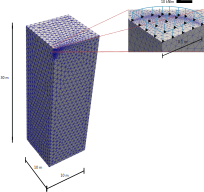
\includegraphics[width=0.75\textwidth]{boussinesq/boussinesq.pdf}
    \caption{Geometry and mesh adopted for the benchmark with a circular distributed load.}
    \label{fig:boussinesq_mesh}
\end{figure}

% ..............................................................................................
\subsection{Materials and numerical parameters}
% ..............................................................................................
The soil is modelled as a one-phase continuum with a linear elastic constitutive law, with the
following parameters:

\begin{itemize}[noitemsep,topsep=0pt,parsep=0pt,partopsep=0pt]
    \item Young's modulus: \qty{20}{\mega\pascal},
    \item Poisson ratio: \qty{0.3}{},
    \item Density: \qty{2000}{\kilogram\per\meter\cubed}.
\end{itemize}


% ----------------------------------------------------------------------------------------------
\section{Results}
% ----------------------------------------------------------------------------------------------
Figure~\ref{fig:boussinesq_results} presents the vertical displacement along the surface of the elastic half-space,
and the vertical stress below the centre of the circular load.
The figure compares the STEM results against the analytical solution.
If follows that there is an agreement between both solutions, demonstrating the accuracy of STEM
for this type of static loading condition.

\begin{figure}[h]
    \centering
    \includegraphics[width=0.8\textwidth]{boussinesq/boussinesq_comparison.pdf}
    \caption{(a) Vertical displacement along the surface of the half-space, (b) vertical stress below the centre of the
    circular load.}
    \label{fig:boussinesq_results}
\end{figure}

% ==============================================================================================
\chapter{Dynamic horizontal point load on dam 2D} \label{ch:vibrating_dam_2D}
% ==============================================================================================

% ----------------------------------------------------------------------------------------------
\section{Introduction}
% ----------------------------------------------------------------------------------------------
This benchmark compares the STEM numerical solution against an analytical solution for the natural frequencies of a 
dam subjected to a dynamic horizontal point load under plane-strain conditions.

The analytical solution is presented in~\cite[Chapter~7.3.4]{Kramer_1996}. The analytical solution provides the first
5 natural frequencies of vibration of the dam structure, which are compared against the numerical model.

% ----------------------------------------------------------------------------------------------
\section{Model Description}
% ----------------------------------------------------------------------------------------------

% ..............................................................................................
\subsection{Geometry, mesh and loading}
% ..............................................................................................
The reference geometry as presented in~\cite{Kramer_1996} is given with feet units. For consistency with the rest of
the benchmarks in this report, the geometry has been converted to SI units (meters).

The soil domain is modeled in 2D and represents a triangle with base \qty{160.02}{\meter} and height \qty{45.72}{\meter},
the left slope is inclined with a ratio of 2:1 (horizontal to vertical), while the right slope is inclined with a ratio
of 1.5:1. The mesh is created with second order triangular elements and uses an average element size of \qty{2}{\meter}.
Figure~\ref{fig:vibrating_dam_mesh} illustrates the geometry and mesh adopted for the analysis.

The horizontal point load with a magnitude of \qty{1e6}{\newton\per\meter} is instantly applied at the top of the dam
structure and is kept constant during the analysed time window.

All nodes along the bottom boundary are fully fixed, while all remaining nodes are constrained to move only in the horizontal 
x direction.

\begin{figure}
    \centering
    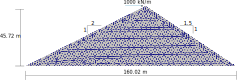
\includegraphics[width=0.75\textwidth]{vibrating_dam/vibrating_dam_mesh.pdf}
    \caption{Geometry and mesh adopted for the vibrating dam benchmark.}
    \label{fig:vibrating_dam_mesh}
\end{figure}

% ..............................................................................................
\subsection{Materials and numerical parameters}
% ..............................................................................................
The soil is modeled as a one-phase continuum with a linear elastic constitutive law, with the
following parameters:

\begin{itemize}[noitemsep,topsep=0pt,parsep=0pt,partopsep=0pt]
    \item Young's modulus: \qty{722}{\mega\pascal},
    \item Poisson ratio: 0.49,
    \item Density: \qty{2000}{\kilogram\per\meter\cubed}.
\end{itemize}

Material damping is excluded from this analysis.

The dynamic analysis is performed over a \qty{2}{\second} time window, with a time step of \qty{0.001}{\second}.
The system of equations is solved using the Newmark time integration~\cite{Newmark_1959} scheme with
parameters $\beta = 0.25$ and $\gamma = 0.5$.

% ----------------------------------------------------------------------------------------------
\section{Results}
% ----------------------------------------------------------------------------------------------
Figure~\ref{fig:vibrating_dam_results} presents the power spectral density of the horizontal displacement of the
 top of the dam.
The figure compares the STEM results against the analytical solution.
The peaks of the power spectral density occur at the expected first five natural frequencies,
showing an agreement between the numerical and analytical solutions.

\begin{figure}[h]
    \centering
    \includegraphics[width=0.8\textwidth]{vibrating_dam/power_spectral_density.pdf}
    \caption{Power spectral density plot of the horizontal displacement at the top of the dam}
    \label{fig:vibrating_dam_results}
\end{figure}


\clearpage
\bibliographystyle{unsrt}
\bibliography{references}

\end{document}
